\newpage
\appendix

\begin{table}[!t]
\begin{tabular}{lll}
$x$ AlwaysPrecedes $y$ &  $x$ NeverFollowedBy $y$    &   $x$ AlwaysFollowedBy $y$ \\
\hline
P, P & C, P & A, TXA \\
P, C & A, P &  \\
P, A & A, TXC & \\
P, TXC & TXC, TXA & \\
P, TXA & TXC, P & \\
C, TXC & TXC, C & \\
A, TXA & TXC, A & \\
& TXA, C & \\
& TXA, P & \\
& TXA, TXC & \\
& TXA, A & \\
\label{table:twopc_invariants}
\end{tabular}

\caption{Temporal invariants mined for the two-phase commit protocol.}
\end{table}

\section{Temporal Invariants Mined for Two-Phase Commit Protocol}
\label{appendix:twopc_invariants}

Table~\ref{table:twopc_invariants} lists all the temporal invariants mined
from valid two-phase commit protocol traces.

\newpage

\begin{figure*}
\centering

\framebox{\subfloat[Calls that generate one or more Status reply
  messages: requesting the public/friend/user time-lines, posting an
  update.]{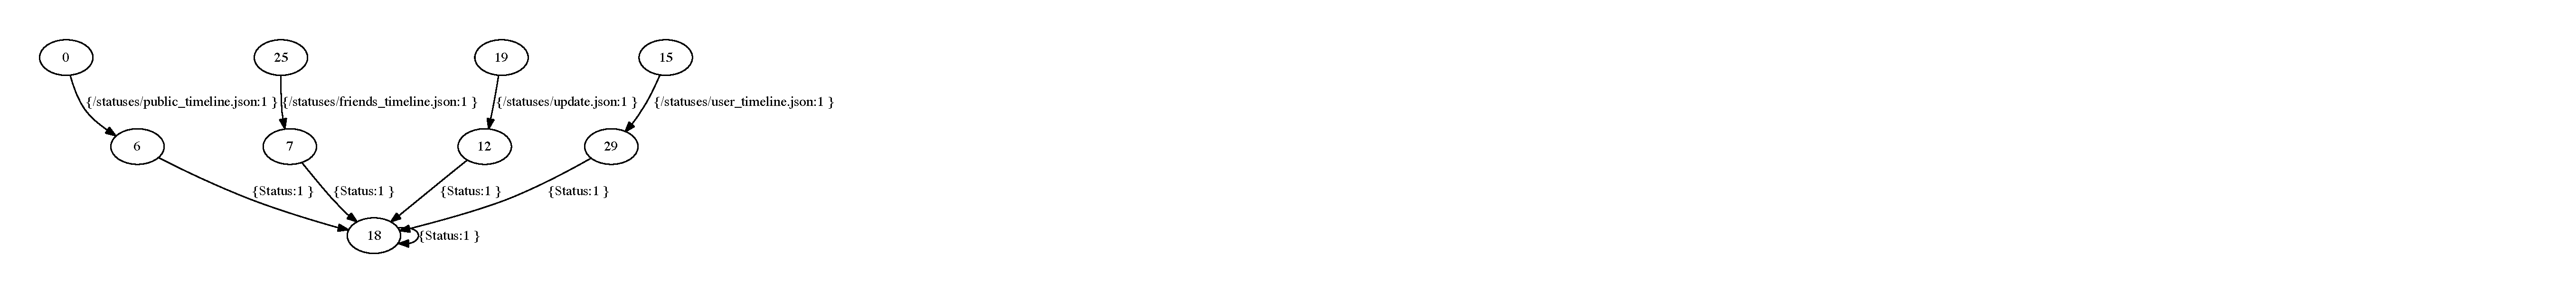
\includegraphics[width=6in]{img/twit_api1.pdf}}}

\framebox{\subfloat[Calls that generate exactly one User reply
  message: update profile, leave/follow a user, test
  503p]{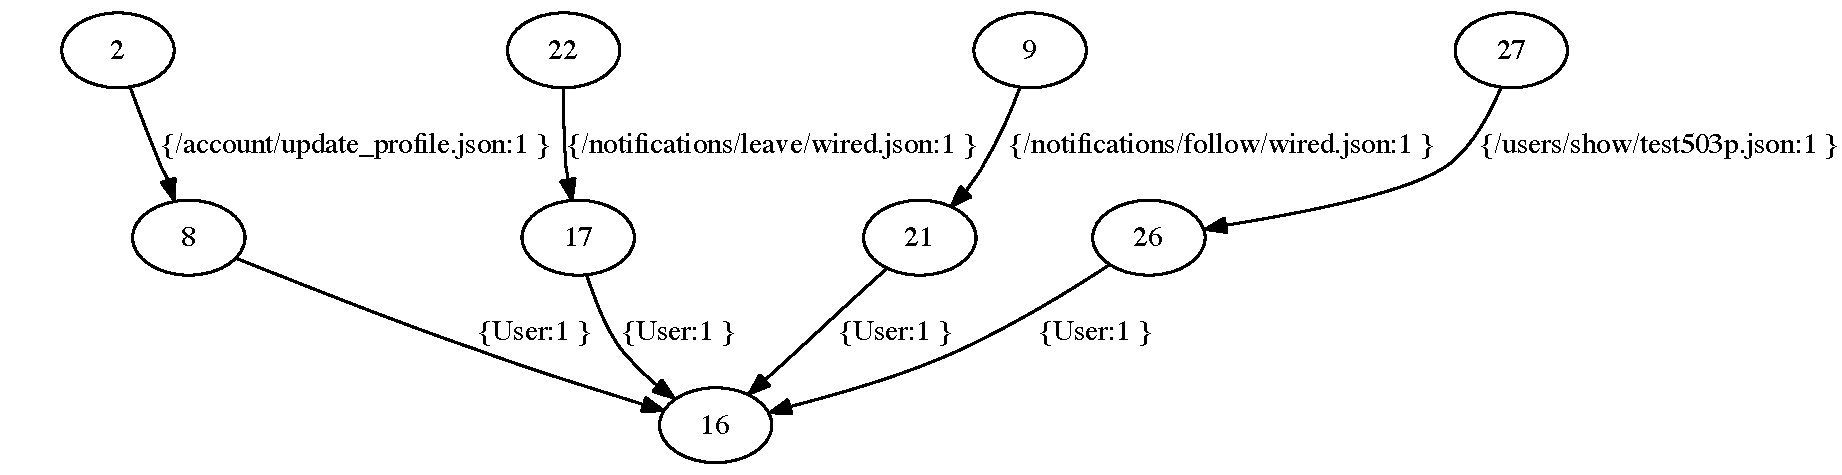
\includegraphics[width=6in]{img/twit_api3.pdf}}}

\framebox{\subfloat[The trends call generates one or more Trend
  reply messages.]{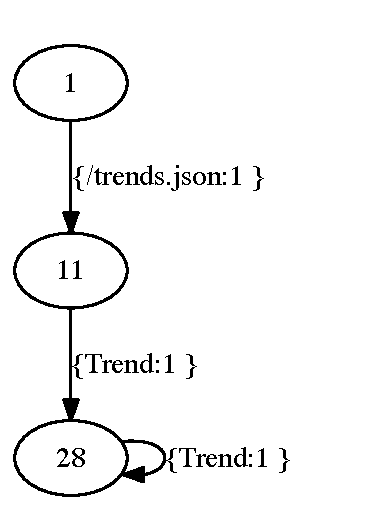
\includegraphics[width=1.3in]{img/twit_api2.pdf}}}
\framebox{\subfloat[Call to search generates at least one Result reply
  message.]{
\includegraphics[width=1.2in]{img/twit_api4.pdf}}}
\framebox{\subfloat[Call to rate limit status generates a single reply.]{
\includegraphics[width=1.6in]{img/twit_api5.pdf}}}
\framebox{\subfloat[Requesting to show a friendship status returns a
  single Relationship message in
  reply.]{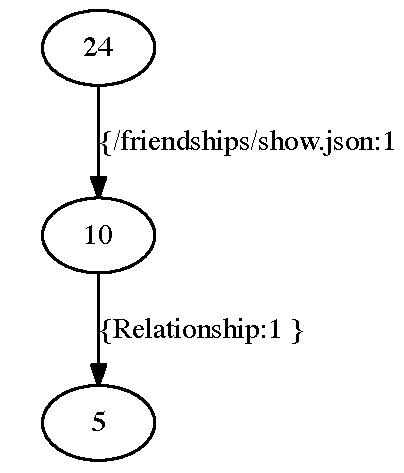
\includegraphics[width=1.5in]{img/twit_api6.pdf}}}

\framebox{\subfloat[Reply to status call does not generate any
  replies.]{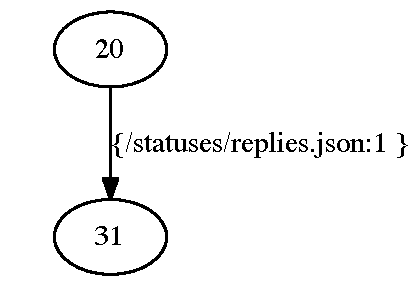
\includegraphics[width=1.5in]{img/twit_api7.pdf}}}

\caption{The collections of state machines \textbf{(a)}-\textbf{(g)}
  depict the various Twitter client API message generating calls and
  respective server replies. Each state machine is a single
  interactions with the server. Generated using Bikon.}
\label{fig:twitter_api}
\end{figure*}

\newpage

\begin{sidewaysfigure*}[p]
% \scalebox{0.8}
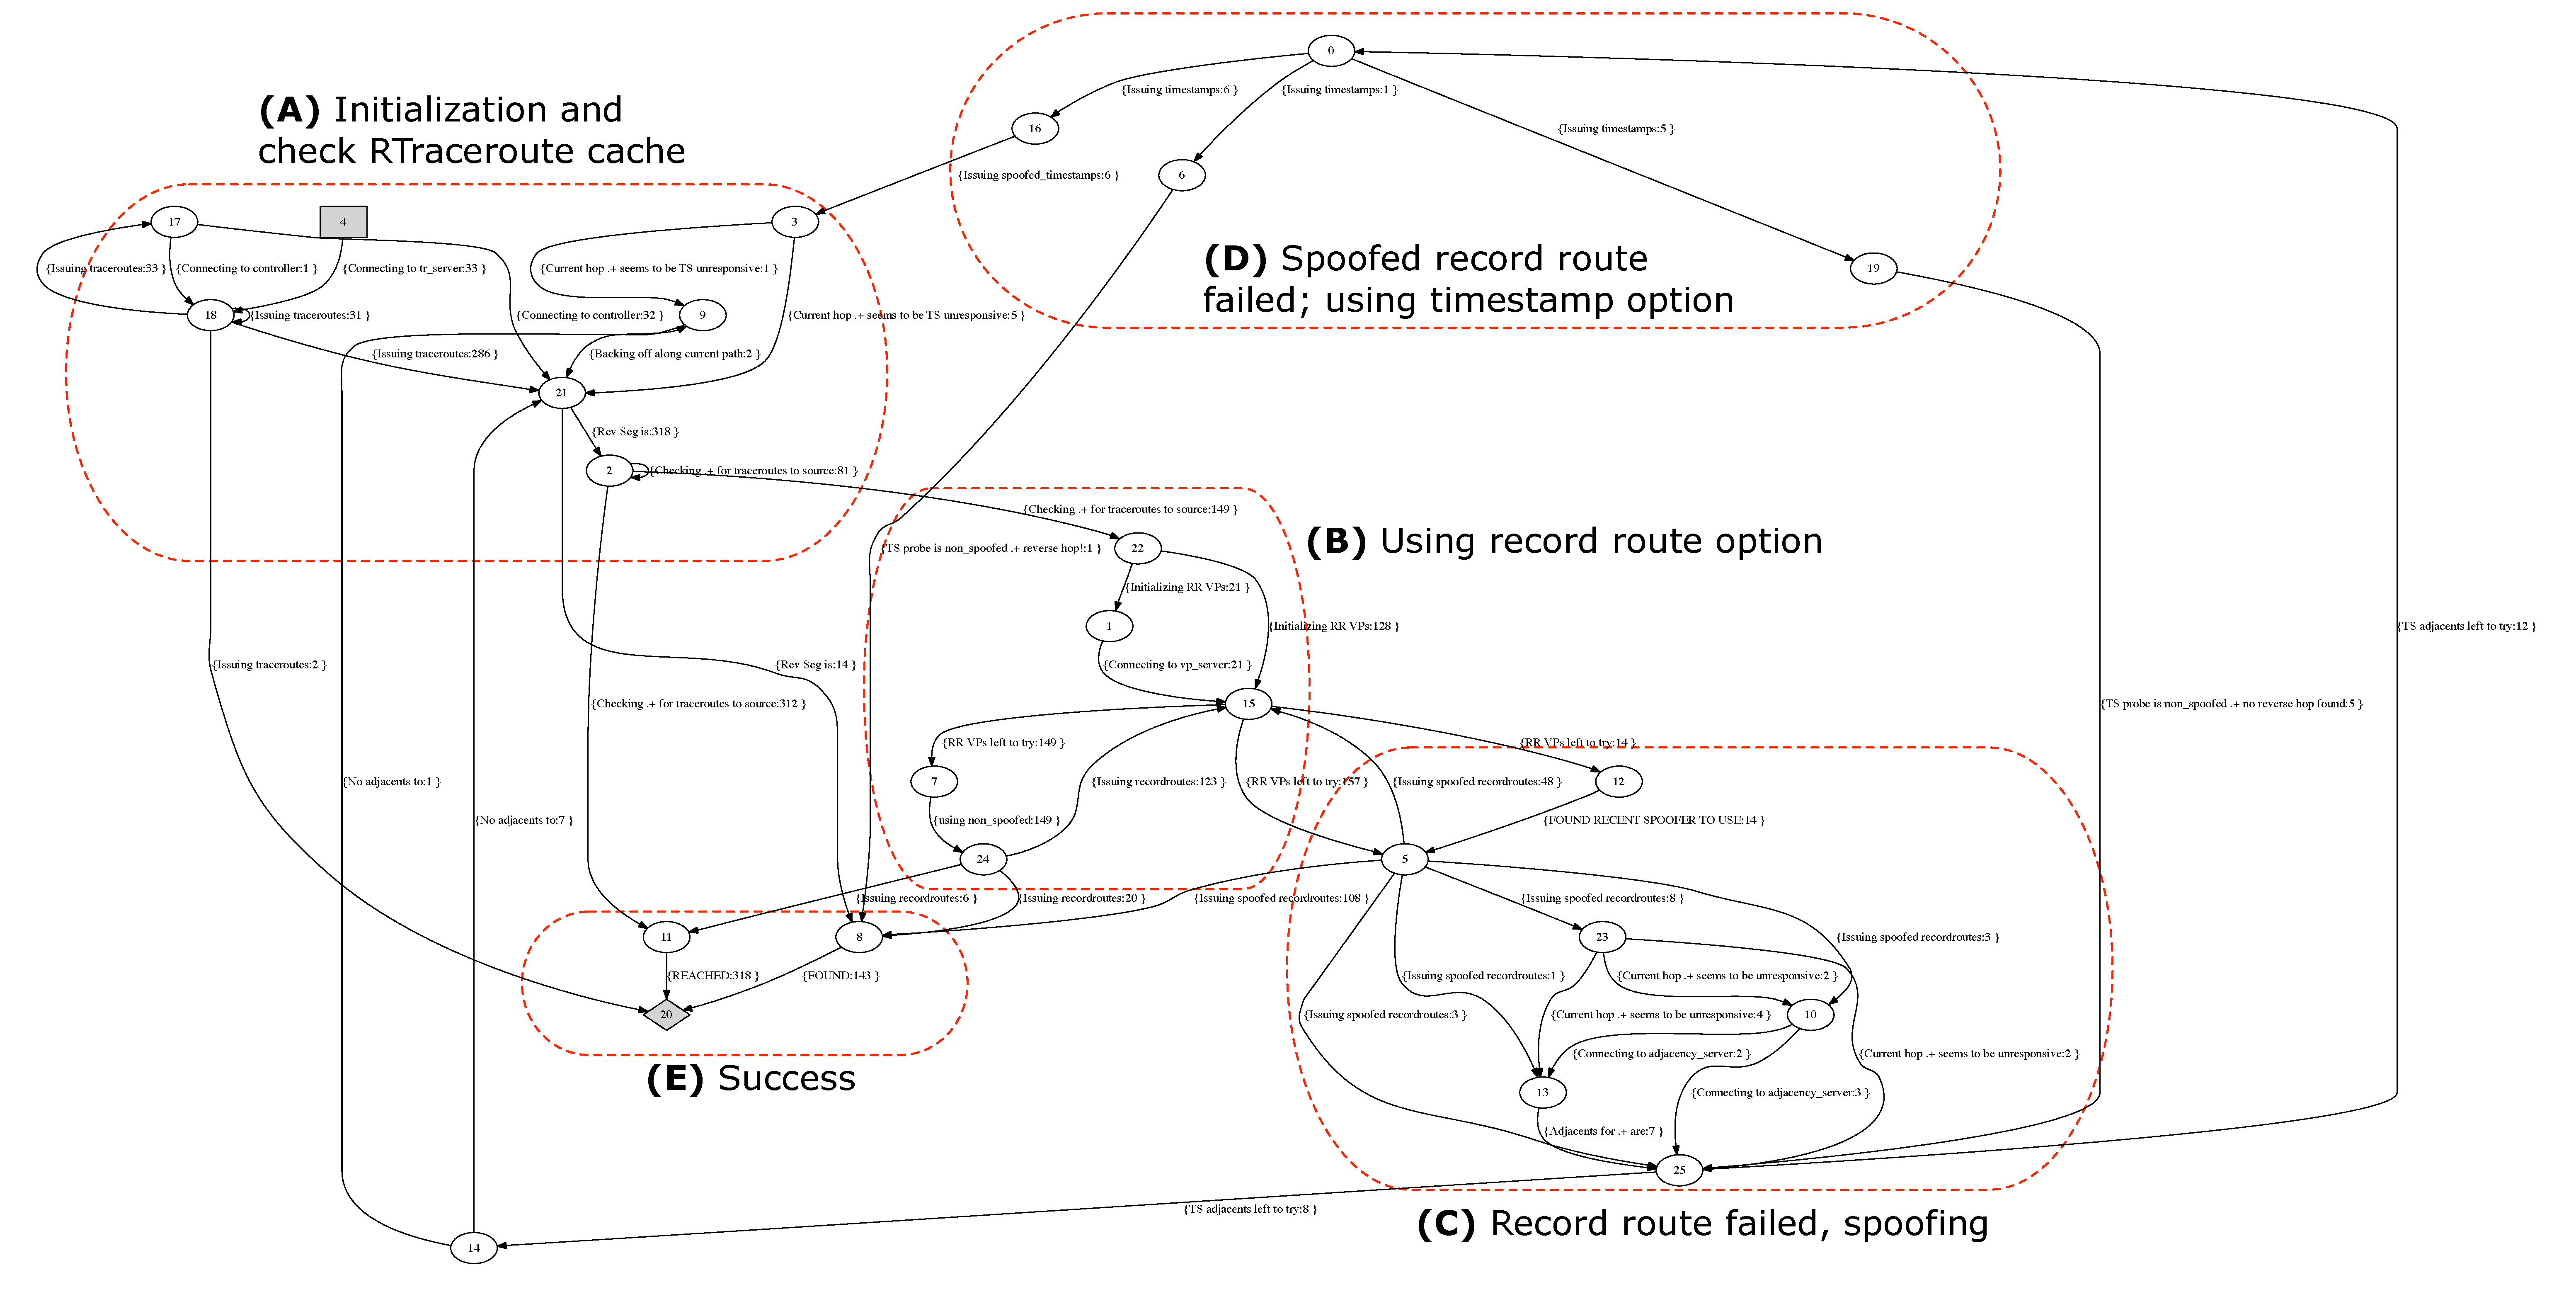
\includegraphics[width=10in,height=7in]{img/multiple_traces_scalable_gktail_labeled.pdf}
\caption{The state machine for the reverse traceroute system. Each
  partition is a computation of a single segment on the reverse path.
  The grey rectangle is the start state, and the grey diamond is the
  terminating state. Generated using GK-Tail. The overlays
  \textbf{(a)} - \textbf{(e)} (specified with red dashed lines) were
  generated by the developer during our user study, and correspond to
  state machines for each type of method the system uses to determine
  a single segment on the reverse path.}
  \label{fig:rt_multiple_traces_scalable_gktail}
\end{sidewaysfigure*}

